\section{SLURM Operation and Services}
\subsection{Command Line Utilities}

The command line utilities are the user interface to SLURM functionality.
They offer users access to remote execution and job control. They also 
permit administrators to dynamically change the system configuration. 
These commands all use SLURM APIs which are directly available for 
more sophisticated applications.

\begin{itemize}
\item {\tt scancel}: Cancel a running or a pending job or job step, 
subject to authentication and authorization. This command can also 
be used to send an arbitrary signal to all processes on all nodes 
associated with a job or job step.

\item {\tt scontrol}: Perform privileged administrative commands
such as draining a node or partition in preparation for maintenance. 
Many \scontrol\ functions can only be executed by privileged users.

\item {\tt sinfo}: Display a summary of partition and node information.
A assortment of filtering and output format options are available.

\item {\tt squeue}: Display the queue of running and waiting jobs 
and/or job steps. A wide assortment of filtering, sorting, and output 
format options are available.

\item {\tt srun}: Allocate resources, submit jobs to the SLURM queue,
and initiate parallel tasks (job steps). 
Every set of executing parallel tasks has an associated \srun\ which 
initiated it and, if the \srun\ persists, managing it. 
Jobs may be submitted for batch execution, in which case 
\srun\ terminates after job submission. 
Jobs may also be submitted for interactive execution, where \srun\ keeps 
running to shepherd the running job. In this case, 
\srun\ negotiates connections with remote {\tt slurmd}'s 
for job initiation and to
get stdout and stderr, forward stdin, and respond to signals from the user.
The \srun\ may also be instructed to allocate a set of resources and
spawn a shell with access to those resources.
\srun\ has a total of 13 parameters to control where and when the job 
is initiated.

\end{itemize}

\subsection{Plugins}

In order to make the use of different infrastructures possible, 
SLURM uses a general purpose plugin mechanism. 
A SLURM plugin is a dynamically linked code object which is 
loaded explicitly at run time by the SLURM libraries. 
A plugin provides a customized implemenation of a well-defined
API connected to tasks such as authentication, interconnect fabric, 
task scheduling.
A common set of functions is defined for use by all of the different 
infrastructures of a particular variety. 
For example, the authentication plugin must define functions 
such as: 
{\tt slurm\_auth\_activate} to create a credential,
{\tt slurm\_auth\_verify} to verify a credential to 
approve or deny authentication, 
{\tt slurm\_auth\_get\_uid} to get the user ID associated with 
a specific credential, etc.
It also must define the data structure used, a plugin type, 
a plugin version number.
The available plugins are defined in the configuration file.
%When a slurm daemon is initiated, it reads the configuration 
%file to determine which of the available plugins should be used. 
%For example {\em AuthType=auth/authd} says to use the plugin for 
%authd based authentication and {\em PluginDir=/usr/local/lib} 
%identifies the directory in which to find the plugin.

\subsection{Communications Layer}

SLURM presently uses Berkeley sockets for communications. 
However, we anticipate using the plugin mechanism to easily 
permit use of other communications layers. 
At LLNL we are using an Ethernet for SLURM communications and 
the Quadrics Elan switch exclusively for user applications. 
The SLURM configuration file permits the identification of each 
node's hostname as well as its name to be used for communications. 
%In the case of a control machine known as {\em mcri} to be 
%communicated with using the name {\em emcri} (say to indicate 
%an ethernet communications path), this is represented in the 
%configuration file as {\em ControlMachine=mcri ControlAddr=emcri}.
%The name used for communication is the same as the hostname unless 
%%otherwise specified.

While SLURM is able to manage 1000 nodes without difficulty using 
sockets and Ethernet, we are reviewing other communication 
mechanisms which may offer improved scalability. 
One possible alternative is STORM\cite{STORM01}. 
STORM uses the cluster interconnect and Network Interface Cards to 
provide high-speed communications including a broadcast capability. 
STORM only supports the Quadrics Elan interconnnect at present, 
but does offer the promise of improved performance and scalability. 

\subsection{Security}

SLURM has a simple security model: 
Any user of the cluster may submit parallel jobs to execute and cancel
his own jobs.  Any user may view SLURM configuration and state
information.  
Only privileged users may modify the SLURM configuration,
cancel any jobs, or perform other restricted activities.  
Privileged users in SLURM include the users {\em root} 
and {\tt SlurmUser} (as defined in the SLURM configuration file). 
If permission to modify SLURM configuration is 
required by others, set-uid programs may be used to grant specific
permissions to specific users.

We presently support three authentication mechanisms via plugins: 
{\tt authd}\cite{Authd02}, {\tt munged} and {\tt none}. 
A plugin can easily be developed for Kerberos or authentication 
mechanisms as desired.
The \munged\ implementation is described below.
A \munged\ daemon running as user {\em root} on each node confirms the 
identify of the user making the request using the {\tt getpeername} 
function and generates a credential. 
The credential contains a user ID, 
group ID, time-stamp, lifetime, some pseudo-random information, and 
any user supplied information. The \munged\ uses a private key to 
generate a Message Authentication Code (MAC) for the credential.
The \munged\ then uses a public key to symmetrically encrypt 
the credential including the MAC. 
SLURM daemons and programs transmit this encrypted 
credential with communications. The SLURM daemon receiving the message 
sends the credential to \munged\ on that node. 
The \munged\ decrypts the credential using its private key, validates it 
and returns the user ID and group ID of the user originating the 
credential.
The \munged\ prevents replay of a credential on any single node 
by recording credentials that have already been authenticated.
In SLURM's case, the user supplied information includes node 
identification information to prevent a credential from being 
used on nodes it is not destined for.

When resources are allocated to a user by the controller, a 
{\em job step credential} is generated by combining the user ID, job ID, 
step ID, the list of resources allocated (nodes), and the credential
lifetime. This job step credential is encrypted with 
a \slurmctld\ private key. This credential 
is returned to the requesting agent ({\tt srun}) along with the
allocation response, and must be forwarded to the remote {\tt slurmd}'s 
upon job step initiation. \slurmd\ decrypts this credential with the
\slurmctld 's public key to verify that the user may access
resources on the local node. \slurmd\ also uses this job step credential 
to authenticate standard input, output, and error communication streams. 

%Access to partitions may be restricted via a {\em RootOnly} flag.  
%If this flag is set, job submit or allocation requests to this 
%partition are only accepted if the effective user ID originating 
%the request is a privileged user. 
%The request from such a user may submit a job as any other user. 
%This may be used, for example, to provide specific external schedulers
%with exclusive access to partitions.  Individual users will not be 
%permitted to directly submit jobs to such a partition, which would 
%prevent the external scheduler from effectively managing it.  
%Access to partitions may also be restricted to users who are 
%members of specific Unix groups using a {\em AllowGroups} specification.

\subsection{Job Initiation}

There are three modes in which jobs may be run by users under SLURM. The
first and most simple is {\em interactive} mode, in which stdout and
stderr are displayed on the user's terminal in real time, and stdin and
signals may be forwarded from the  terminal transparently to the remote
tasks. The second is {\em batch} mode, in which the job is
queued until the request for resources can be satisfied, at which time the
job is run by SLURM as the submitting user. In {\em allocate} mode,
a job is allocated to the requesting user, under which the user may
manually run job steps via a script or in a sub-shell spawned by \srun .

\begin{figure}[tb]
\centerline{\epsfig{file=../figures/connections.eps,scale=0.5}}
\caption{\small Job initiation connections overview. 1. The \srun\ connects to
         \slurmctld\ requesting resources. 2. \slurmctld\ issues a response,
         with list of nodes and job credential. 3. The \srun\ opens a listen
         port for every task in the job step, then sends a run job step
         request to \slurmd . 4. \slurmd 's initiate job step and connect
         back to \srun\ for stdout/err. }
\label{connections}
\end{figure}

Figure~\ref{connections} gives a high-level depiction of the connections
that occur between SLURM components during a general interactive job
startup.
The \srun\ requests a resource allocation and job step initiation from the {\tt slurmctld},
which responds with the job ID, list of allocated nodes, job credential.
if the request is granted.
The \srun\ then initializes listen ports for each
task and sends a message to the {\tt slurmd}'s on the allocated nodes requesting
that the remote processes be initiated. The {\tt slurmd}'s begin execution of
the tasks and connect back to \srun\ for stdout and stderr. This process and
the other initiation modes are described in more detail below.

\subsubsection{Interactive mode initiation}

\begin{figure}[tb]
\centerline{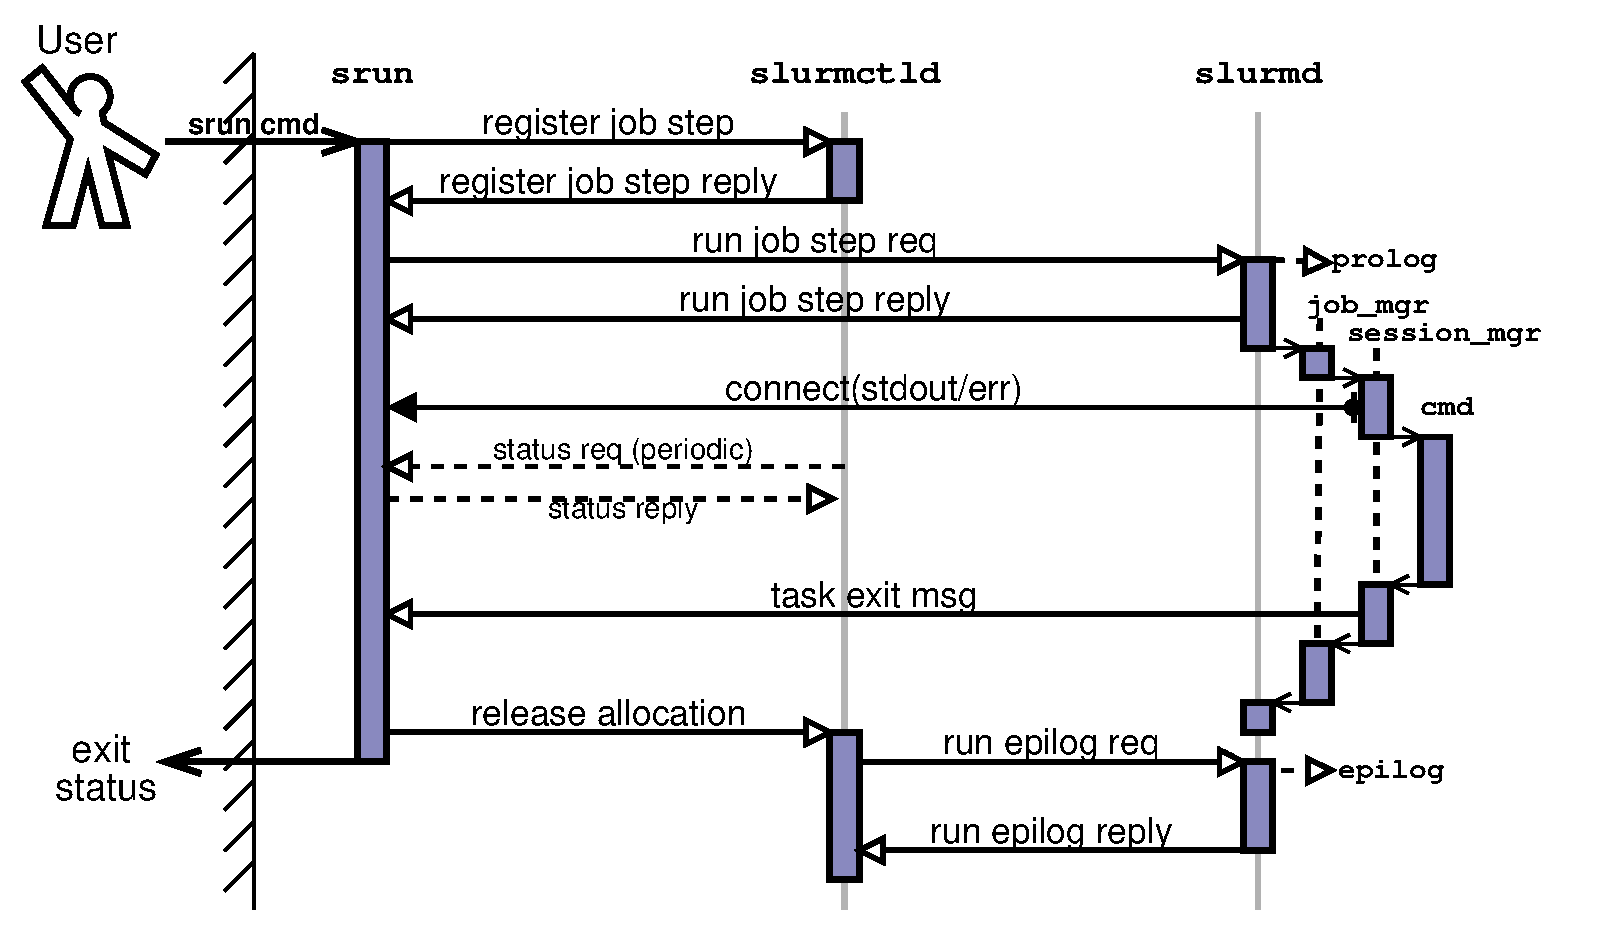
\epsfig{file=../figures/interactive-job-init.eps,scale=0.5} }
\caption{\small Interactive job initiation. \srun\ simultaneously allocates
nodes
         and a job step from \slurmctld\ then sends a run request to all
         \slurmd 's in job. Dashed arrows indicate a periodic request that
         may or may not occur during the lifetime of the job.}
\label{init-interactive}
\end{figure}

Interactive job initiation is illustrated in Figure~\ref{init-interactive}.
The process begins with a user invoking \srun\ in interactive mode.
In Figure~\ref{init-interactive}, the user has requested an interactive
run of the executable ``{\tt cmd}'' in the default partition.

After processing command line options, \srun\ sends a message to
\slurmctld\ requesting a resource allocation and a job step initiation.
This message simultaneously requests an allocation (or job) and a job step.
The \srun\ waits for a reply from {\tt slurmctld}, which may not come instantly
if the user has requested that \srun\ block until resources are available.
When resources are available
for the user's job, \slurmctld\ replies with a job step credential, list of
nodes that were allocated, cpus per node, and so on. The \srun\ then sends
a message each \slurmd\ on the allocated nodes requesting that a job
step be initiated. The \slurmd 's verify that the job is valid using
the forwarded job step credential and then respond to \srun .

Each \slurmd\ invokes a job thread to handle the request, which in turn
invokes a task thread for each requested task. The task thread connects
back to a port opened by \srun\ for stdout and stderr. The host and
port for this connection is contained in the run request message sent
to this machine by \srun . Once stdout and stderr have successfully
been connected, the task thread takes the necessary steps to initiate
the user's executable on the node, initializing environment, current
working directory, and interconnect resources if needed.

Once the user process exits, the task thread records the exit status and
sends a task exit message back to \srun . When all local processes
terminate, the job thread exits. The \srun\ process either waits
for all tasks to exit, or attempt to clean up the remaining processes
some time after the first task exits.
Regardless, once all
tasks are finished, \srun\ sends a message to the \slurmctld\ releasing
the allocated nodes, then exits with an appropriate exit status.

When the \slurmctld\ receives notification that \srun\ no longer needs
the allocated nodes, it issues a request for the epilog to be run on each of
the \slurmd 's in the allocation. As \slurmd 's report that the epilog ran
successfully, the nodes are returned to the partition.


\subsubsection{Batch mode initiation}

\begin{figure}[tb]
\centerline{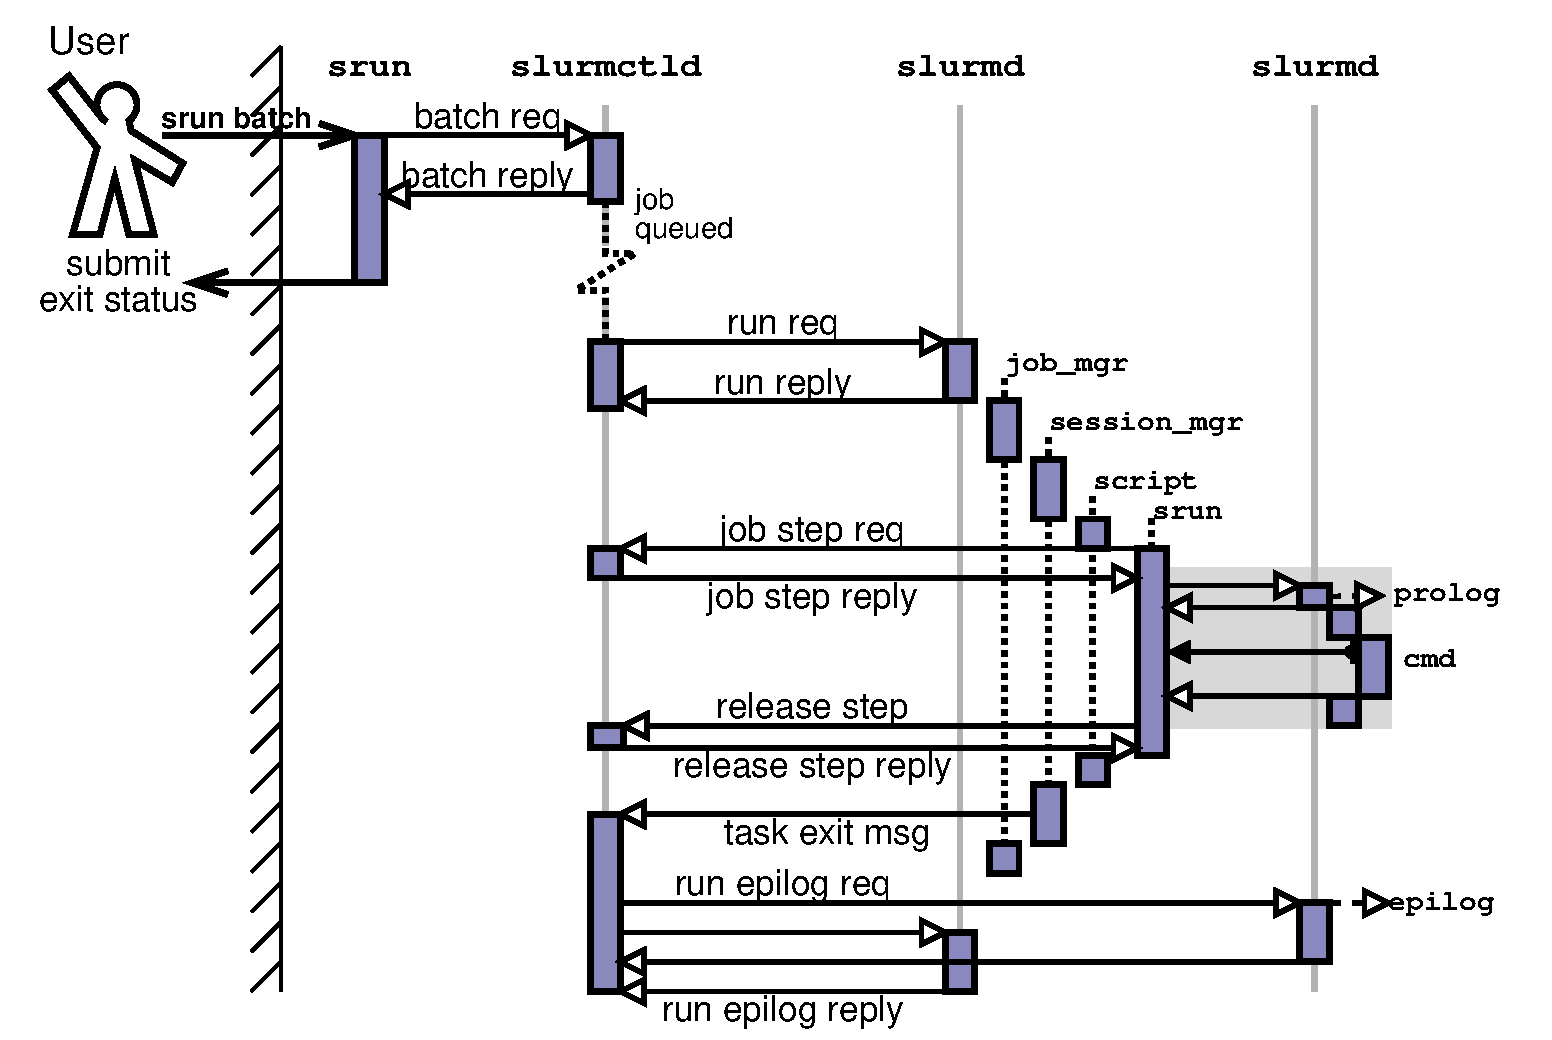
\epsfig{file=../figures/queued-job-init.eps,scale=0.5} }
\caption{\small Queued job initiation.
         \slurmctld\ initiates the user's job as a batch script on one node.
         Batch script contains an srun call which initiates parallel tasks
         after instantiating job step with controller. The shaded region is
         a compressed representation and is illustrated in more detail in the
         interactive diagram (Figure~\ref{init-interactive}).}
\label{init-batch}
\end{figure}

Figure~\ref{init-batch} illustrates the initiation of a batch  job in SLURM.
Once a batch job is submitted, \srun\ sends a batch job request
to \slurmctld\ that contains the input/output location for the job, current
working directory, environment, requested number of nodes. The
\slurmctld\ queues the request in its priority ordered queue.

Once the resources are available and the job has a high enough priority,
\slurmctld\ allocates the resources to the job and contacts the first node
of the allocation requesting that the user job be started. In this case,
the job may either be another invocation of \srun\ or a {\em job script} which
may have multiple invocations of \srun\ within it. The \slurmd\ on the remote
node responds to the run request, initiating the job thread, task thread,
and user script. An \srun\ executed from within the script detects that it
has access to an allocation and initiates a job step on some or all of the
nodes within the job.

Once the job step is complete, the \srun\ in the job script notifies the
\slurmctld\, and terminates. The job script continues executing and may
initiate further job steps. Once the job script completes, the task
thread running the job script collects the exit status and sends a task exit
message to the \slurmctld . The \slurmctld\ notes that the job is complete
and requests that the job epilog be run on all nodes that were allocated.
As the \slurmd 's respond with successful completion of the epilog,
the nodes are returned to the partition.

\subsubsection{Allocate mode initiation}

\begin{figure}[tb]
\centerline{\epsfig{file=../figures/allocate-init.eps,scale=0.5} }
\caption{\small Job initiation in allocate mode. Resources are allocated and
         \srun\ spawns a shell with access to the resources. When user runs
         an \srun\ from within the shell, the a job step is initiated under
         the allocation.}
\label{init-allocate}
\end{figure}

In allocate mode, the user wishes to allocate a job and interactively run
job steps under that allocation. The process of initiation in this mode
is illustrated in Figure~\ref{init-allocate}. The invoked \srun\ sends
an allocate request to \slurmctld , which, if resources are available,
responds with a list of nodes allocated, job id, etc. The \srun\
process spawns a shell on the user's terminal with access to the
allocation, then waits for the shell to exit at which time the job
is considered complete.

An \srun\ initiated within the allocate sub-shell recognizes that it
is running under an allocation and therefore already within a job. Provided
with no other arguments, \srun\ started in this manner initiates a job
step on all nodes within the current job. However, the user may select
a subset of these nodes implicitly.

An \srun\ executed from the sub-shell reads the environment and
user options, then notify the controller that it is starting a job step
under the current job. The \slurmctld\ registers the job step and responds
with a job credential. The \srun\ then initiates the job step using the same
general method as described in the section on interactive job initiation.

When the user exits the allocate sub-shell, the original \srun\ receives
exit status, notifies \slurmctld\ that the job is complete, and exits.
The controller runs the epilog on each of the allocated nodes, returning
nodes to the partition as they complete the epilog.
